%%%%%%%%%%%%%%%%%%%%%%%%%%%%%%%%%%%%%%%%%%%%%%%%%%%%%%%%%%%%%%%%%%
\section{Distributed Mesh Management}  
%%%%%%%%%%%%%%%%%%%%%%%%%%%%%%%%%%%%%%%%%%%%%%%%%%%%%%%%%%%%%%%%%%

A distributed mesh data structure is an infrastructure executing 
underneath providing all parallel mesh-based operations needed to support
parallel adaptive analysis. An efficient and scalable distributed mesh data structure is
 mandatory to achieve performance since it strongly influences
the overall performance of adaptive mesh-based simulations. In addition to
the general mesh-based operations, the distributed
mesh data structure must support $(i)$ efficient communication between
 entities duplicated over multiple processes, $(ii)$ migration of entities
 between processes, and $(iii)$ dynamic load balancing. 

This chapter presents the concept and functionalties of distributed mesh management. $\S$\ref{pmodel} describes a partition model that is developed in FMDB for the purpose of effectively meeting the specific functionalities of distributed meshes~\cite{seolthesis, fmdb06}. The readers not interested in the internal design and implementation of the distributed meshes in FMDB might skip $\S$\ref{pmodel}

%%%%%%%%%%%%%%%%%%%%%%%%%%%%%%%%%%%%%%%%%%%%
% SECTION 4.1	
\subsection{Distributed Mesh Representation}  
%%%%%%%%%%%%%%%%%%%%%%%%%%%%%%%%%%%%%%%%%%%%

\begin{figure}
\centering
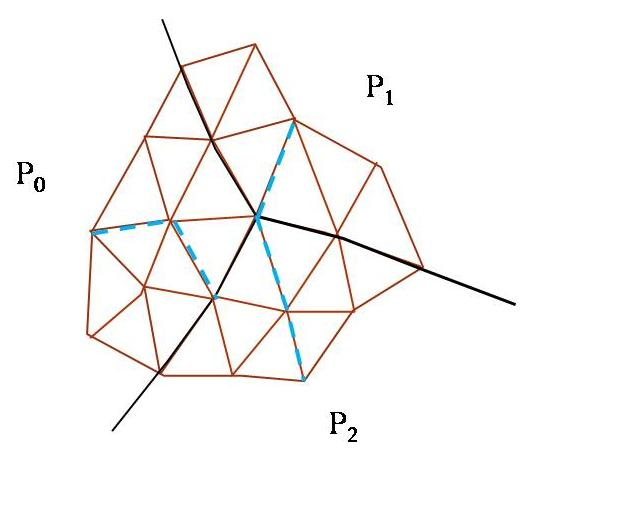
\includegraphics[width=3in]{../fig/distMesh1.jpg}
\caption[Distributed mesh on three processes with two parts per process]{Distributed mesh on three processes $P_0$, $P_1$ and $P_2$ with two parts per each process}
\label{distMesh1}  % the \label command comes AFTER the caption
\end{figure}

\emph{A distributed mesh} is a mesh divided into parts for distribution
over a set of processes for specific reasons, for example, parallel computation.

\begin{description}
\item[Definition 3.1] \emph{Part}\\
A part consists of the set of mesh entities assigned to a
process. For each part, a unique global part id within an entire system and a local part id within a process can be given.
\end{description}

Each part will be treated as a serial mesh with the addition of mesh
part boundaries to describe groups of mesh entities that are on inter-part boundaries. Mesh entities on part boundaries are
duplicated on all parts on which they are used in adjacency relations. Mesh entities not on the part boundary exist on only one part and referred as \emph{internal entities}. In implementation, for effective manipulation of multiple parts on each process, a single mesh data is defined on each process so multiple parts are contained in the mesh data where the mesh data is assigned to a process. The mesh data defined on each process is referred as \emph{mesh instance}. Figure~\ref{distMesh1} depicts a mesh that is distributed on 6 parts where the mesh instance on each process has two parts respectively. The dashed lines are \emph{part boundaries} within a process and the solid black lines are \emph{part boundaries} between the processes. The vertices and edges on part boundaries are duplicated on multiple parts.

In order to simply denote a set of parts where a mesh entity physically exist, termed \emph{residence part set}, we define an operator {\RP}. 

\begin{description}
\item[Definition 3.2] \emph{Residence part set operator \RP\Ls\Mdi\Rs} \\
An operator that returns a set of global part id(s) where \Mdib exists. 
\end{description}

%For any entity \Mdi\blk not on the boundary of any other mesh entities and on partition
%$p$, \RP\Ls\Mdi\Rs\blk returns \{$p$\} since when the entity is not on the boundary of any
%other mesh entities of higher order, its bounding part is determined
%simply to be the partition where it resides.  For entity \Mdi\blk on the
%boundary of higher order mesh entities, \RP\Ls\Mdi\Rs\blk is determined by the
%resident partition equation.

\begin{description}
\item[Definition 3.3] \emph{Residence part equation of \Mdi} \\
If \{$M^d_i$\{$M^q$\}\} $= \emptyset$, $d<q$, \RP$[$\Mdi\Rs\blk = \{$p$\} where $p$
is the id of a part where $M^d_i$ exists. Otherwise, \RP$[$\Mdi\Rs\blk = $\cup$ \RP$[$$M^q_j$ $\mid$ $M^d_i$ $\in$
\{$\partial$($M^q_j$)\}\Rs. %\\
%: For entity $M^q_k$, every \Mdib $\in$ \{$\partial$($M^q_k$)\} is on \RP\Ls$M^q_k$\Rs.
%Therefore, \Mdib exists wherever the mesh entity, $M^q_k$, it bounds exists.
\end{description}

For any entity \Mdi\blk not on the part boundary of any higher order mesh entities and on part
$p$, \RP$[$\Mdi\Rs\blk returns \{$p$\} since when the entity is not on the boundary of any
other mesh entities of higher order, its residence part set is determined simply to be the part where it resides.
If entity \Mdi\blk is on the boundary of other higher order mesh entities, \Mdi\blk is duplicated on multiple parts depending on the residence part set of its bounding entities since \Mdib exists wherever a mesh entity it bounds exists.

Therefore, the residence part set of \Mdi\blk is the union
of residence part set of all entities that it bounds. For a mesh topology
where the entities of order $d>0$ are 
bounded by entities of order $d-1$, \RP\Ls\Mdi\Rs\blk is determined to be
\{p\} if \{\Mdi\{\Mdpok\}\} $= \emptyset$. Otherwise, \RP\Ls\Mdi\Rs\blk is $\cup$ \RP\Ls$M^{d+1}_k$ $\mid$
$M^d_i$ $\in$ \{$\partial$($M^{d+1}_k$)\}\Rs. For instance, for the
3D non-manifold mesh depicted in Figure~\ref{pmesh3procs}, where $M^3_1$ and $M^2_1$
are on $P_0$, $M^3_2$ and $M^2_2$ are on $P_1$ and $M^1_1$ is on $P_2$, residence part set of $M^0_1$ are \{$P_0$, $P_1$, $P_2$\} since the union of residence part set of its bounding
edges, \{$M^1_1$, $M^1_2$, $M^1_3$, $M^1_4$, $M^1_5$, $M^1_6$\}, are \{$P_0$, $P_1$,
$P_2$\}. 

\begin{figure}
\centering
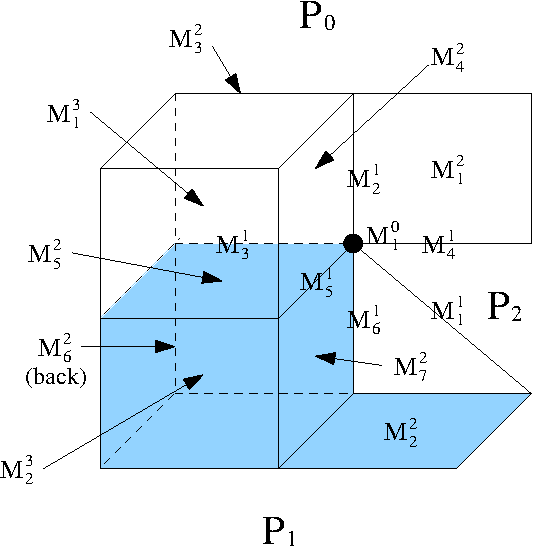
\includegraphics[width=2.5in]{../fig/PO}
\caption{Example 3D mesh distributed on three parts}
\label{pmesh3procs}  
\end{figure}

To migrate mesh entities to other parts, the destination part id's of
mesh entities must be specified before moving the mesh
entities. The residence part set equation implies that once the destination
part id of a \Mdi\blk that is not on its boundary of any other
mesh entities is set, the other entities needed to migrate are determined by
the entities it bounds. Thus, a mesh entity that is not on the boundary of any higher order mesh entities is the basic
unit to assign the destination part id in the mesh migration procedure.
 
\begin{description}
\item[Definition 3.4] \emph{Partition object}\\
The basic unit to which a destination part id is assigned. The full set of partition objects is
the set of mesh entities that are not part of the boundary of any higher order mesh
entities. In a 3D mesh, this includes all mesh regions, the mesh faces not bounded
by any mesh regions, the mesh edges not bounded by any mesh faces or regions, and mesh vertices not
bounded by any mesh edges, faces or regions. A set of unique mesh entities refered as entity set can also be a partition object if designated to be a migration unit.
\end{description}

In case of a manifold model, partition objects are all mesh
regions in 3D and all mesh faces in 2D. In case of a non-manifold model, the careful
lookup for entities not being bounded is required 
over the entities of one specific dimension. For example, partition objects of the mesh in Figure~\ref{pmesh3procs} are
$M^1_1$, $M^2_1$, $M^2_2$, $M^3_1$, and $M^3_2$. 

%%%%%%%%%%%%%%%%%%%%%%%%%%%%%%%%%%%%%%
\subsection{Functional Requirements}\label{ch:distmesh:req} 
%%%%%%%%%%%%%%%%%%%%%%%%%%%%%%%%%%%%%%

\subsubsection{Communication links}

Mesh entities on the part boundaries (shortly, part boundary entities) must be aware of where they are duplicated. 

\begin{description}
\item[Definition 3.5] \emph{Remote part}\\
Non-self part\footnote{A part that is not in the current local
part} where a mesh entity is duplicated.
\item[Definition 3.6] \emph{Remote copy}\\
Non-owned part boundary entities, in other words, the memory location of a mesh entity duplicated on remote part. 
\end{description}

\subsubsection{Ownership}

In parallel adaptive analysis, the mesh and its partitioning can change thousands of time
during the simulation~\cite{adapt06, deCougny-Shephard99, Oliker-etal00, Shep-etal97}. Therefore, at the mesh functionality 
level, an efficient mechanism to update the mesh partitioning and keep the links
between parts updated are mandatory to achieve scalability.

For entities on part boundaries duplicated on multiple parts, it is beneficial to
assign a specific part as the owner with charge of modification, communication or computation of the copies. For the purpose of simple denotation, a part bounday entity owned by the self part is referred as \emph{owner} of other entities copied on other parts.

\begin{figure}
\centering
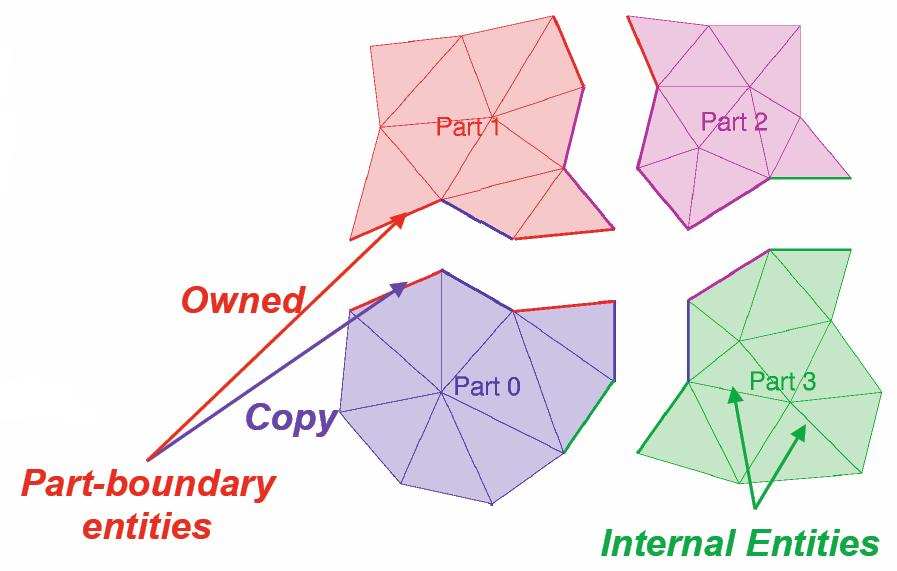
\includegraphics[width=3.5in]{../fig/distMesh2.jpg}
\caption[A distributed mesh on four processes with one part per process]{A distributed mesh on four processes with one part per process~\cite{itapsweb}}
\label{distMesh2}  % the \label command comes AFTER the caption
\end{figure}

Figure~\ref{distMesh2} depicts a mesh that is distributed on four processes with a single part per process. Entities on part boundaries are either of owner or copies. Internal entities are owners.

\subsubsection{Ghosting}

To avoid communications between the parts, it is beneficial to support the ability to have a copy of non-part boundary entities on other part, referred as $ghosting$~\cite{itapsweb}.

\begin{description}
\item[Definition 3.7] \emph{Ghost copy or ghost entity}\\
Non-owned, non-part-boundary entity in a part
\end{description}

\begin{figure}
\centering
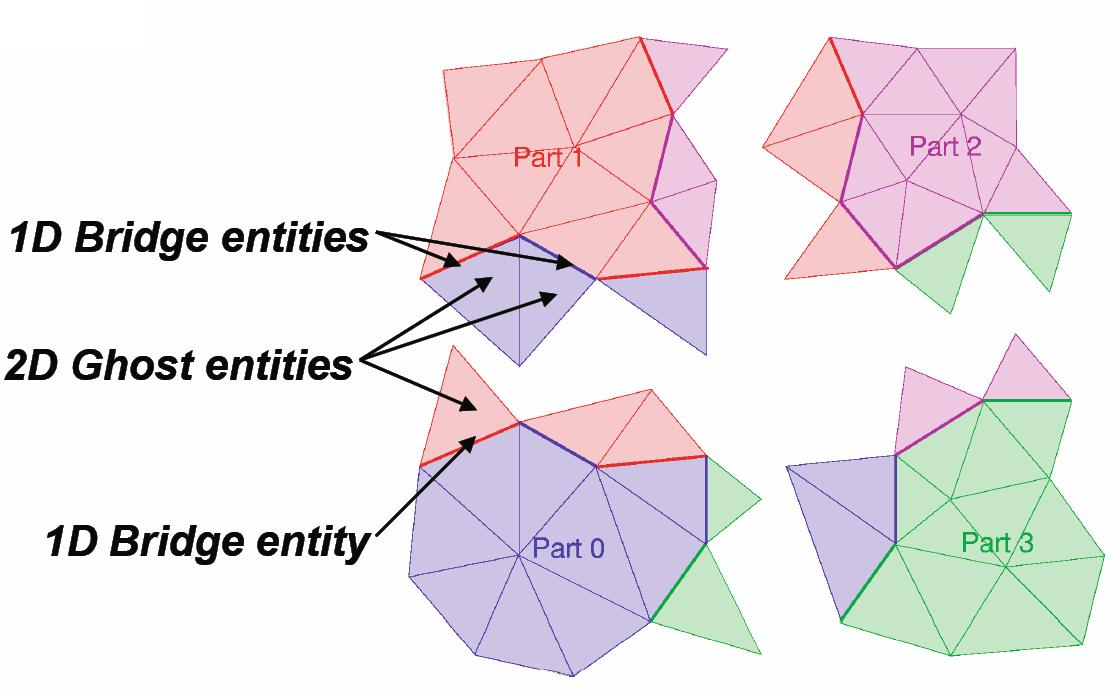
\includegraphics[width=3.7in]{../fig/ghost2.jpg}
\caption[A distributed mesh on four parts with ghost entities]{A distributed mesh on four parts with ghost entities~\cite{itapsweb}}
\label{ghost}  % the \label command comes AFTER the caption
\end{figure}

Figure~\ref{ghost} depicts a distributed mesh on four parts with ghost entities along the part boundaries. Similar to ownership of part boundary entities, the original owner entity is designated as \emph{owner} of all ghost copies.

To perform a layer-based ghosting, four input parameters are needed:
\begin{itemize}
\item bridge (entity) dimension
\item ghost (entity) dimension
\item the number of layers
\item a true/false flag indicating whether to include non-owned part boundary entities will be included for bridge entities. If true, all part boundary entities of bridge dimension are considered to construct ghost layer(s). If false, only $owned$ part boundary entities of bridge dimension are considered.
\end{itemize}

Ghost entities are specified through a \emph{bridge} dimension.  The number of layers is measured from the inter-part interfaces.  For example, to get two layers of region entities in the ghost layer, measured from faces on the interface, bridge dimension, ghost dimention, and the number of layers shall be, respectively, 2, 3, 2. The number of layers specified is with respect to the global mesh, that is, ghosting may extend beyond a single neighboring process if the number of layers is high.

In Figure~\ref{ghost}, The input parameters of ghosting (bridge dimension, ghost dimension, the number of layers and a flag) are $[1, 2, 1, true]$.

\begin{figure}
\centering
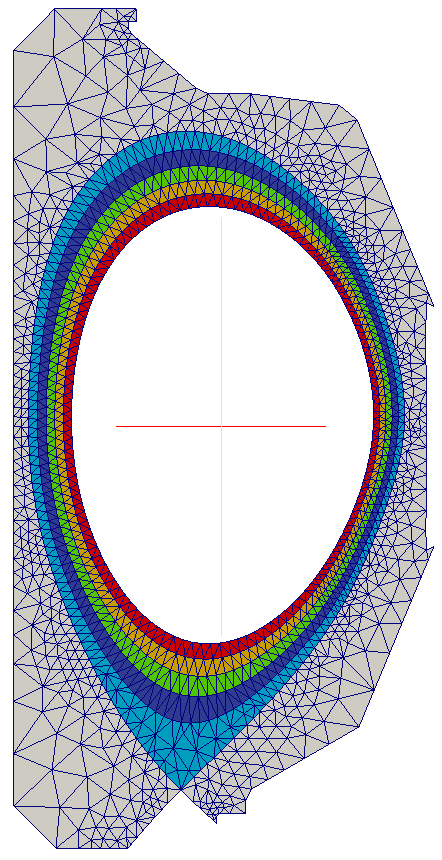
\includegraphics[width=1.5in]{./fig/part17-22.png}\hspace{1cm}
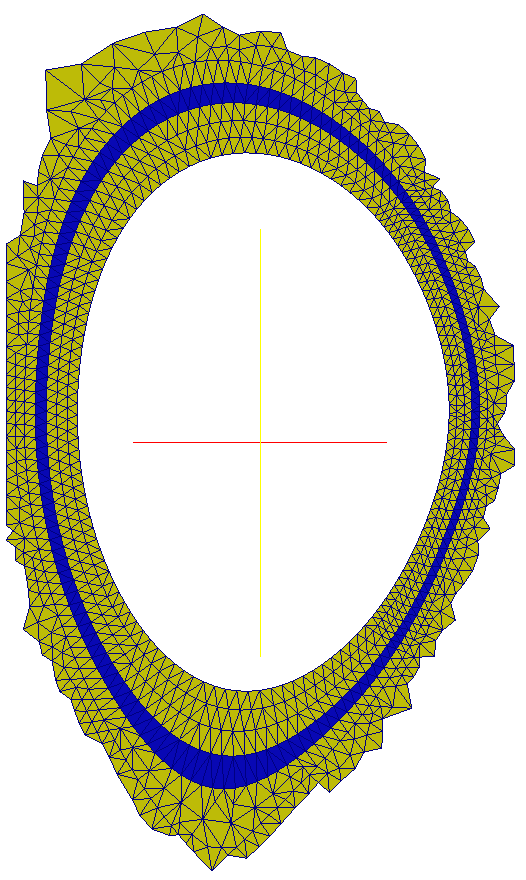
\includegraphics[width=1.7in]{./fig/part20-ghosted-copy}\hspace{1cm}
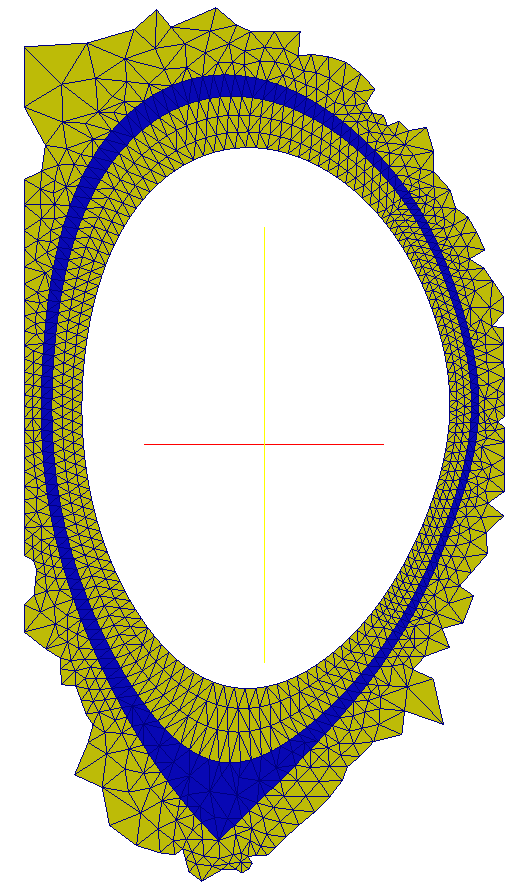
\includegraphics[width=1.7in]{./fig/part21-ghosted-copy}\hspace{1cm}
\caption{3-layer ghosting: (left to right) initial 6-part mesh, part 3 with 3 ghost layers, and part 4 with 3 ghost layers}
\label{xgc}  % the \label command comes AFTER the caption
\end{figure}

The left figure in Figure~\ref{xgc} depicts 6-part distributed mesh. The parts 0 to 5 are colored in red, orange, green, blue, turquoise, and gray respectively. The middle and right figure in Figure~\ref{xgc} illustrate the part 3 and part 4 with 3 ghost layers, where the original mesh entities are colored in blue and the ghost copies are colored in yellow. The input parameters of ghosting procedure are $[0, 2, 3, true]$.

%%%%%%%%%%%%%%%%%%%%%%%%%%%%%%%%%%%%%%%%%%%%
\subsubsection{Migration} 
%%%%%%%%%%%%%%%%%%%%%%%%%%%%%%%%%%%%%%%%%%%%

For effective management of distributed mesh with multiple parts per process, the following migration procedures are needed.

\begin{itemize}
\item Migrating entities and entity sets between parts with tag
\item Migrating whole parts between processes
\item Redistributing mesh. For example, splitting $n$ part mesh to $m$ parts, $n$ $\neq$ $m$, to load the mesh on an $m$ process machine.
\end{itemize}

%%%%%%%%%%%%%%%%%%%%%%%%%%%%%%%%%%%%%%%%%%%%
% SECTION 4.2
\subsection{A Partition Model}\label{pmodel}
%%%%%%%%%%%%%%%%%%%%%%%%%%%%%%%%%%%%%%%%%%%%

\begin{figure}
\centering
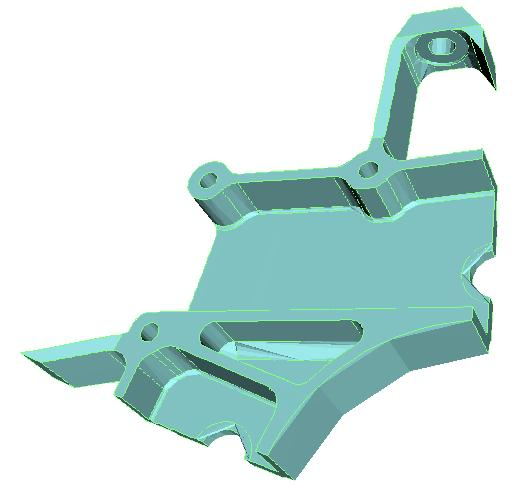
\includegraphics[width=1.9in]{../fig/hub_model.jpg}
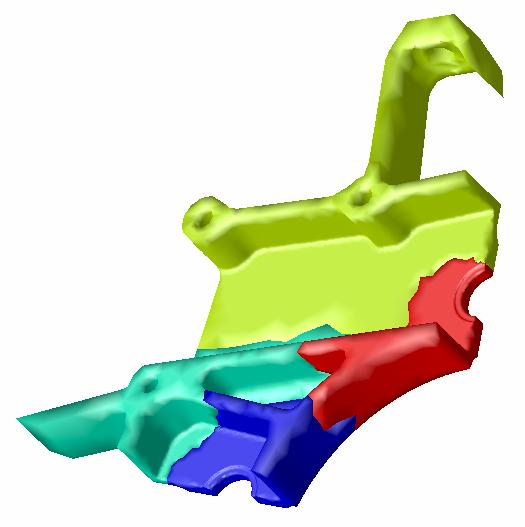
\includegraphics[width=1.9in]{../fig/hub_np4_pmodel.jpg}
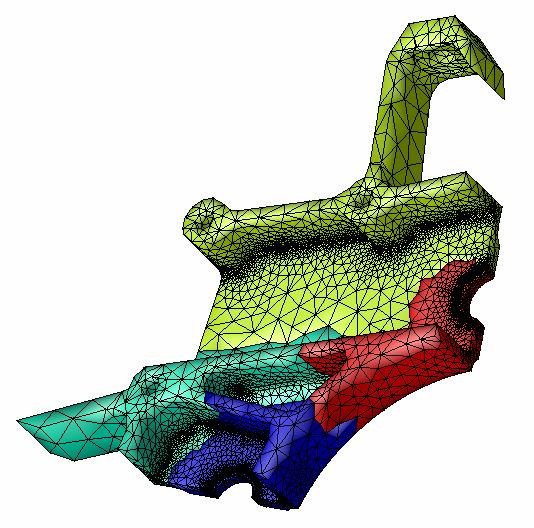
\includegraphics[width=1.9in]{../fig/hub_np4.jpg}
\caption[Hierarchy of domain decomposition]{Hierarchy of domain decomposition: (left to right) geometry model, partition model, and distributed mesh on 4 processes}
\label{torus}
\end{figure}

To meet the goals and functionalities of distributed meshes, a partition model has been
developed between the mesh and the geometric model. As illustrated in
Figure~\ref{torus}, the partition model can be
viewed as a part of hierarchical domain 
decomposition. Its purpose is to represent mesh
partitioning in topology and support mesh-level parallel 
operations through inter-part boundary links with ease. 

The specific implementation is the parallel extension of the unstructured mesh representation, such that standard mesh entities and adjacencies are used on processes only with the addition of the partition entity information needed to support all operations across multiple processes.

The partition model introduces a set of topological entities that represents the collections of mesh entities based on their location with
respect to the partitioning. Grouping mesh entities to define a partition entity
can be done with multiple criteria based on the level of functionalities and needs of distributed meshes. These constructs are consistent with the ITAPS iMeshP specification~\cite{itapsweb}.

At a minimum, \emph{residence part set} must be a criterion to be
able to support the inter-part communications. \emph{Connectivity} between entities is also desirable for a criterion to
support operations quickly and can be used optionally. Two mesh entities are $connected$ if they are on the same part and reachable via adjacency operations. The  connectivity is expensive but useful in representing separate  chunks in a part. It enables diagnoses of the quality of mesh partitioning immediately at the partition model level. In our implementation, for the efficiency purpose, only residence part set is used for the criterion. 

\begin{description}
\item[Definition 2.8] \emph{Partition (model) entity}\\
A topological entity in the partition model, \Pdi, which
represents a group of mesh entities of dimension $d$, that have the
same \RP. Each partition model entity is uniquely determined by \RP. 
\end{description}

Each partition model entity stores dimension, id, residence part set, and
the owning part. From a mesh entity level, by keeping proper relation to the
partition model entity, all needed services to represent mesh partitioning and support
inter-part communications are easily supported. 

\begin{description}
\item[Definition 2.9] \emph{Partition classification}\\
The unique association of mesh topological entities of dimension \di, \Mdii, to the topological entity of the
partition model of dimension \djj, \Pdjjb where $d_i \le d_j$, on which it lies is termed partition
classification and is denoted \Mdiib\clasb $P^{d_j}_j$.

\item[Definition 2.10] \emph{Reverse partition classification}\\
For each partition entity, the set of equal order mesh entities classified on that
entity defines the reverse partition classification for the partition model
entity. The reverse partition classification
is denoted as RC(\Pdj) = \{\Mdib $\mid$ \Mdib\clasb\Pdj\}. 
\end{description}

Figure~\ref{fig:pmeshwithpclas} illustrates a 3D distributed mesh with mesh entities labeled
with arrows indicating the partition classification of the entities onto the
partition model entities and its associated partition model. The mesh
vertices and edges on the thick black lines are classified on
partition edge $P^1_1$. The mesh
vertices, edges and faces on the shaded
planes are classified on the partition faces pointed with each arrow. The remaining
mesh entities are non-part boundary 
entities, therefore they are classified on the partition regions. Note the reverse
classification returns only the same order mesh entities. The reverse partition classification of
$P^1_1$ returns mesh edges located 
on the thick black lines, and the reverse partition classification of partition
face $P^2_i$ returns mesh faces on the shaded planes.

\begin{figure}
\centering
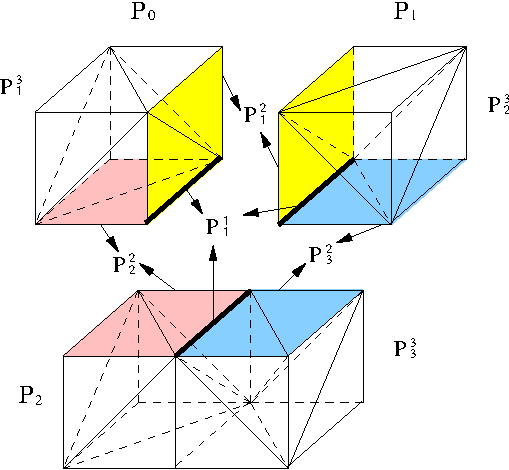
\includegraphics[height=2.5in]{../fig/pmesh3Dpclas2}\hspace{.3in}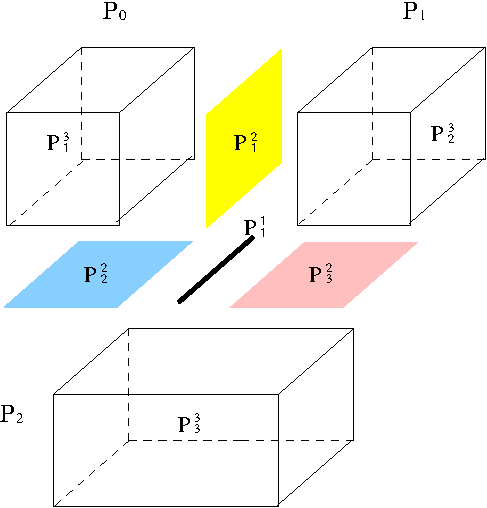
\includegraphics[height=2.5in]{../fig/pmodel3D}\\
\vspace{5pt}(a) distributed mesh \hspace{1in}(b) partition model\\
\vspace{7pt}
\caption{Distributed mesh and its association with the partition model via partition classifications}
\label{fig:pmeshwithpclas}
\end{figure}

